\section{Materials and Methods}
\subsection{Study Site}
Pismo State Beach Monarch Butterfly Grove (hereafter "Pismo") is located in San Luis Obispo County, California (35.12940° N, 120.628° W). The site encompasses approximately 5 hectares (12.4 acres) and is characterized by a mature grove of blue gum eucalyptus (\textit{Eucalyptus globulus}). The grove is situated approximately 0.5 km from the Pacific Ocean, which lies directly to the west.

The grove's eucalyptus trees are the dominant vertical feature in the local landscape. To the west, between the Pacific Ocean and Pismo, lies the North Beach Campground and Pismo Beach Golf Course, both minimally developed with scattered trees and open grassy areas. The northern and eastern boundaries are adjacent to medium-density residential neighborhoods with single and two-story buildings. To the south extends the Oceano Dunes Natural Preserve State Park, characterized by mature coastal dune scrub habitat with low rolling dunes and perennial vegetation. The site is managed by California State Parks.

% Discuss other trees, heights of trees, and surrounding features. 
% Include figure of the surounding area with a digital surface model. Highlight Pismo Grove with a boundary and show that the areas around the site are relatively flat. Maybe contours? I think it would be interesting to also show height above ground colored to really sell that Pismo is the dominant vertical feature

\subsection{Site Selection Rationale}
Pismo was selected as the primary study site for several key characteristics. The site consistently supports one of the largest aggregations of overwintering monarch butterflies (\textit{Danaus plexippus}) in California, routinely ranking among the top ten overwintering sites by population size \autocite{westernmonarchcount2023}. Even during years of low monarch abundance, such as 2024, Pismo maintains a presence of butterflies while many other sites remain vacant.

The site's physical characteristics make it particularly suitable for wind analysis. The western exposure to the Pacific Ocean provides an unobstructed wind corridor, minimizing confounding topographical effects. The surrounding terrain is predominantly flat, and nearby anthropogenic structures do not exceed two stories in height, representing less than 20\% of the canopy height of the grove's mature eucalyptus trees.

Additionally, Pismo's extensive history of monarch butterfly research and consistent population monitoring provides valuable historical context for this study. The site's well-documented population counts, conducted at regular intervals, offer opportunities for correlating wind patterns with butterfly abundance and distribution patterns.

\subsection{Data Loggers}

- To monitor wind conditions within the grove, twelve anememoters, or wind meters, were installed at various locations within the Pismo grove.
- We used RainWise WindLog Wind Data Loggers for this project. 
- % Cite? https://rainwise.com/windlog-wind-data-logger?srsltid=AfmBOopJ8CFlyo--3fLTENd9DyErLXyfILiOy4HykPw5W-xP4TwHZxaV
- anemomoter sensor locations were mounted to trees nondestructively through the use of tie down straps and metal wire. The locations were selected opportunistically based on what could be accessed via a cherry picker and professional arborist team. Sensor locations were chosen to have varying heights (add range of heights here) and locations within the grove. Care was taken to ensure that no anemometers overhanged areas where pedestrians would walk, incase one were to fall. 
- wind meters were programmed to collect infomation on average wind speed, maximum gusts, and wind direction every minute. 
- wind meters were deployed for two monarch overwintering seasons, 2023-2024, and 2024-2025. 
- % Include exact start and end dates here
- For the 2023 season, sensor issues resulted in several meters having reading issues at various times throughout the sampling period. Data was cleaned and only periods of time that have complete, or near complete observations were used in the analysis. 
- Each sensor had a unique identifer
- In additional to installed wind meters, data was scraped from nearby personal stations through the website, weatherunderground
- Data was scrapped every 15 seconds at a number of nearby stations (name stations). In addition, historical records were also downloaded for each station.
- % Probably need to elaborate on this more. Will be easier once data clean up is done. 
- % Include diagram of how sensors were mounted to tree?
- % Need figure showing sensor locations within the grove. Consider a top down view as well as a cross sectional view showing the variation in heights. 


\subsection{Data Cleaning}
- For each wind meter, a separate SQLite file was created to keep measuresments separate. database files followed the name of the sensor. 
- Using Python, I combined all data into a single dataframe.
% mention how data was excluded or included
% show a timeline of how much complete data exists. Perhaps color coded by percent complete. 


%\begin{figure}[htbp]
%    \centering
%    \textbf{Study Area}\\[1ex]
%    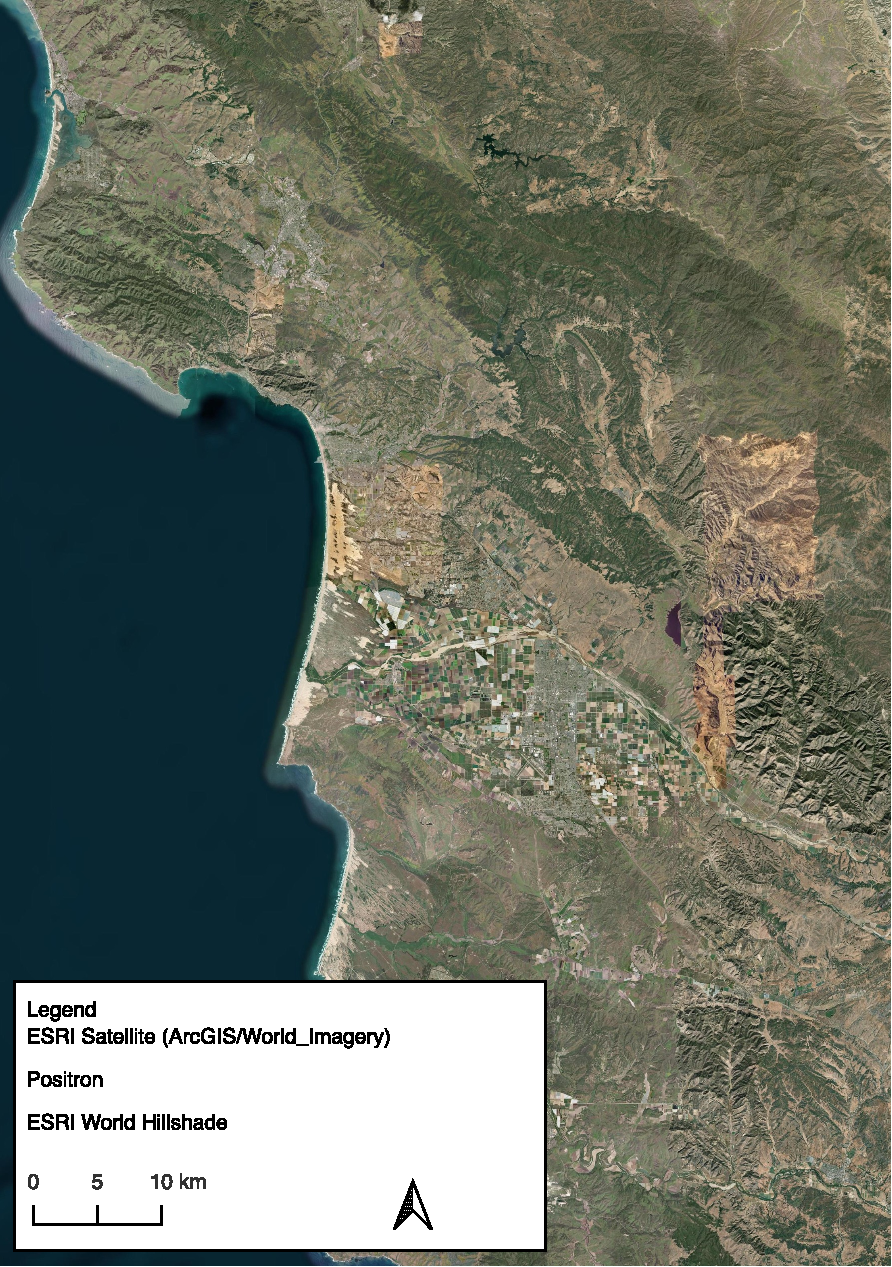
\includegraphics[width=\textwidth]{figures/test.pdf}
%    \caption{Clear, descriptive caption explaining what the figure shows and its significance.}
%    \label{fig:your-label}
%\end{figure}